\section{Linear Approximation}

In the following question, we will implement linear approximation in PyTorch. If you feel you need a refresher of Pytorch concepts and functionality please consult the \href{https://colab.research.google.com/drive/1BZ89PnXpzN2US_OxwuQCazucmuTpuIfS?usp=sharing}{Pytorch Tutorial} we have made available. It is worth noting that the functions you implement in this section will be used in future questions of this assignment. Therefore, in order to avoid the loss of points, please ensure you that your implementation passes the basic test cases we have provided in ~grader.py~ for this question.

Outside of checking the tests within ~grader.py~ you can also test the performance of your implementation locally on the test environment \textbf{using your computer's CPU} by running:

\begin{lstlisting}
$ python run.py --config_filename=q5_linear
\end{lstlisting} 

\begin{enumerate}[(a)]

	\input{05-linear-approximation/01-network-update-rule}

	\item \points{5b}
Implement the ~initialize_models~ function in ~submission/q5_linear_torch.py~ which will define our linear model for both the Q-network and the target network.

	\item \points{5c}
Implement the ~get_q_values~ function in ~submission/q5_linear_torch.py~ to output Q-values for a particular state and network.

	\item \points{5d}
Implement the ~update_target~ function in ~submission/q5_linear_torch.py~ in order to update the target network with the Q-network weights.

	\item \points{5e}
Implement the ~calc_loss~ function in ~submission/q5_linear_torch.py~ which will define our loss function.

	\item \points{5f}
Implement the ~add_optimizer~ function in ~submission/q5_linear_torch.py~ which will define our optimizer.

	\item \points{5g}

In this question, our grader will evaluate the performance of your linear implementation on the test environment based on the code you have already developed in previous questions in this section (No additional code needs to be written for this question).

If you would like, you can observe the performance metrics of your model through running the following command:

\begin{lstlisting}
$ python run.py --config_filename=q5_linear
\end{lstlisting}

This should train your linear model on the test environment with the configuration defined in ~config/q5_linear.yml~. You may view the evaluation scores from your training run under the following directory ~results/q5_linear/~. We expect your implementation to achieve the optimal return on the test environment. Below we have provided a plot of scores which we expect the scores generated by your implementation to closely resemble:

\begin{figure}[H]
\centering
  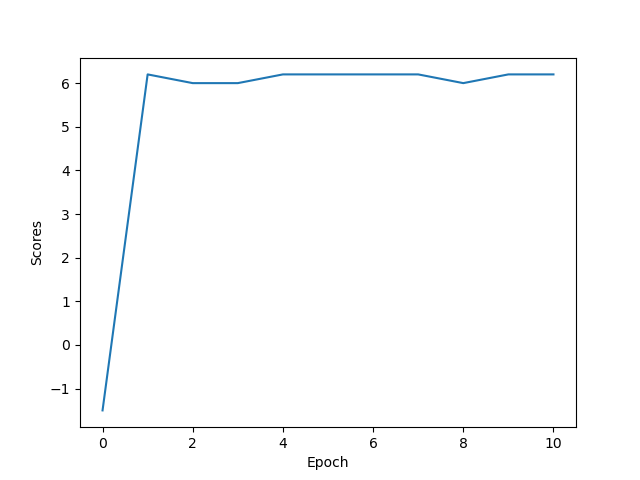
\includegraphics[width=.5\linewidth]{images/linear_test.png}
\end{figure}

\textit{Note: You will be need these results to provide responses to future questions which are made available online via Gradescope.}
\clearpage

\end{enumerate}